\documentclass[12pt]{article}
\usepackage{geometry}
\geometry{
	letterpaper,
	left=20mm,
	right=20mm,
	top=25mm,
	bottom=30mm,
}
\usepackage{graphicx}
\usepackage{tikz}
\usepackage{tikzscale}
\usepackage{pgfplots}
\usepackage{amsmath,amssymb}
\usepackage{enumitem}
\usepackage{algorithm}
\usepackage{algorithmicx}
\usepackage{algpseudocode}
\usepackage{subcaption}
\usepackage{mathtools}
\usepackage{amsthm}
\usepackage{nccmath} %for fleqn
\makeatletter
\def\verbatim@font{\linespread{1}\normalfont\ttfamily}
\makeatother
\usepackage[breaklinks]{hyperref} 
\hypersetup{
	colorlinks   = true,
	citecolor    = blue
}
\hypersetup{linkcolor=blue}
\usepackage[T1]{fontenc}
\DeclarePairedDelimiter{\ceil}{\lceil}{\rceil}
\mathchardef\mhyphen="2D
\newcommand\makeset{\mathop{make\mhyphen set}}
\newcommand\findset{\mathop{find\mhyphen set}}
\newcommand*{\Comb}[2]{{}^{#1}C_{#2}}
\usepackage{mdframed}
\usepackage{fancyhdr} 
\fancyhf{}
\chead{\courseName}
\lhead{\thepage}  
\rhead{\homeworkName}
\renewcommand{\headrulewidth}{1pt}
\renewcommand{\footrulewidth}{0pt} 
\fancypagestyle{first}{% 
	\fancyhf{} % clear all header and footer fields 
	\chead{
		\small
		} % except the center 
	\renewcommand{\headrulewidth}{0pt} 
	\renewcommand{\footrulewidth}{0pt}
} 
\fancypagestyle{second}{% 
	\fancyhf{} % clear all header and footer fields 
	\chead{} % except the center 
	\renewcommand{\headrulewidth}{0pt} 
	\renewcommand{\footrulewidth}{0pt}
}
\pagestyle{fancy} 
	
\usepackage{xepersian}
\settextfont[
Scale=1.2,
Extension=.ttf, 
Path=../../common/fonts/,
BoldFont=*-BOLD
]{B-NAZANIN}
\setlatintextfont[Scale=1.1]{Times New Roman}
%\setdigitfont[Scale=1.4]{Times New Roman}
\setlength\parindent{0pt}

\newcommand{\courseName}{ارزیابی کارایی سیستم های کامپیوتری}
\newcommand{\courseSemester}{پاییز ۱۴۰۲}
\newcommand{\homeworkName}{راهنمای پروژه اول}
\newcommand{\homeworkDue}{موعد: }

\renewcommand{\baselinestretch}{1.5} 

\begin{document}
	\graphicspath{{../../common/cover/},{img/}}
	\pagenumbering{gobble} 
	\thispagestyle{first}
%\newgeometry{top=2cm}
%\newcommand*{\SSS}{\includegraphics[scale=0.2]{ut}}%
%\newcommand*{\TTT}{\includegraphics[scale=0.2]{fanni}}%
\begin{mdframed}
\begin{minipage}[t]{0.2\textwidth}
	\centering
	
\includegraphics[width=0.6\textwidth]{sharif} \\
%	\vspace{0.2cm}
	\homeworkName
\end{minipage}%
\begin{minipage}[b]{0.59\textwidth}
	\centering
	\courseName \\
	\courseSemester
\end{minipage}%
\begin{minipage}[t]{0.2\textwidth}
	\centering
	
\includegraphics[width=0.6\textwidth]{sharif} \\
	\homeworkDue
\end{minipage}%
\end{mdframed}
%\restoregeometry

	\pagenumbering{arabic}
	\begin{itemize}
	\item[*]
	\textbf{آنچه در این تمرین باید تحول دهید :}
	\\
برای این تمرین شما باید اولاً کد برنامه‌ی شبیه‌سازی را به همراه یک
\lr{$Makefile$}
که اجرا کننده‌ی برنامه‌ی شما است، تحویل دهید. نحوه ی ایجاد
\lr{$Makefile$}
برای سیستم عامل لینوکس در انتهای راهنما آمده است. برنامه‌ی شما باید مقادیر احتمال بلوکه شدن
(\lr{$P_b$})
و احتمال خارج شدن از صف یا همان ددلاین
(\lr{$P_d$})
مشتریان و نیز متوسط تعداد مشتری‌های داخل صف
(\lr{$N_c$})
را با دو روش شبیه‌سازی و تحلیلی و به ازای مقادیر مشخص برای پارامترهای
\lr{$\mu$}
و
\lr{$\theta$}
که از فایل
\lr{$parameters.conf$}
می‌‌خواند و مقادیر 5 و 10 و 15 برای
\lr{$\lambda$}
در دو حالت تتا (زمان انتظار) ثابت و نمایی محاسبه کند و در فایل متنی خروجی چاپ کند. همچنین شما باید دو فایل
\lr{$Excel$}
که حاوی داده های به دست آمده در مورد
\lr{$P_b$}
و
\lr{$P_d$}
و
\lr{$N_c$}
مشتریان در دو روش شبیه‌سازی و تحلیلی به ازای تتای ثابت و تتای نمایی می‌باشد را تحویل دهید. در این فایل‌ها مقادیر خطای مطلق و خطای نسبی بین مقادیر حاصل از روش شبیه‌سازی و روش تحلیلی محاسبه می‌شود و به ازای هر روش، سه نمودار رسم میشود. هر قدر خطای شما کمتر باشد و نمودارهای
مقادیر حاصل از روش شبیه سازی و تحلیلی بیشتر بر هم انطباق بیشتری داشته باشند، نمره‌ی بهتری خواهید گرفت.
    \item[*]
	\textbf{آنچه در این تمرین باید به دست آورید :}
	\\
    برای این که بتوانید مقادیر مورد نیاز را برای آن دو فایل \lr{$Excel$} که در بالا ذکر شد به دست آورید، لازم است برنامه‌ای که شما برای خودتان اجرا می‌کنید
    \lr{$P_b$} و \lr{$P_d$} و \lr{$N_c$} 
    را به ازای 
    \lr{$\lambda$} از
    \lr{$0.1$} تا 
    \lr{$20.0$}
    و با پرش \lr{$0.1$}
    محاسبه کند و مقادیر حاصل از روش شبیه‌سازی و تحلیلی مربوط را به ازای تتای ثابت و تتای نمایی در فایل‌های متنی خروجی (ترجیحا به شکل ستونی) چاپ کند تا شما بتوانید
این مقادیر را در ستون‌های مربوطه در فایل \lr{$Excel$} کپی کنید و آن فایل‌ها را تکمیل نمایید.
    \item[*]
	\textbf{ساختار برنامه (قسمت شبیه‌سازی) :}
	\\
	برای انجام شبیه‌سازی، لازم است که شما ابتدا برای مشتریان سیستم و نیز رخدادهای موجود در سیستم ، نوع داده تعریف کنید.
نوع داده‌ی مشتری باید شامل صفاتی از جمله زمان ورود ، زمان انتظار ، زمان سرویس و یک شماره برای مشتری باشد.
    نوع داده‌ی رخداد نیز باید شامل صفاتی از جمله نوع رخداد (3 نوع : ورود مشتری، خارج شدن مشتری از صف یا همان ددلاین و
خارج شدن مشتری از سرور) ، زمان وقوع رخداد و نیز شماره‌ی مشتری مربوط به آن رخداد باشد.
    \\
سپس لازم است که شما لیست مشتریان را تعریف کنید. برای این منظور در یک حلقه‌ی تکرار که به تعداد مشتریان شما تکرار می‌شود، هر مشتری را در یک خانه از یک ساختمان داده از نوع داده‌ی مشتری تعریف می‌کنید. می‌توانید زمان ورود اولین مشتری را صفر در نظر بگیرید سپس برای هریک از مشتریان بعدی، یک عدد تصادفی با توزیع نمایی بر اساس فرمول زیر تولید کنید و با زمان ورود مشتری قبلی جمع کنید و به عنوان زمان ورود مشتری فعلی در نظر بگیرید. همچنین برای تعریف زمان سرویس هر مشتری،
می‌توانید از فرمول زیر استفاده کنید با این تفاوت که به جای
\lr{$\lambda$}
 ، پارامتر
 \lr{$\mu$}
 را قرار دهید تا عددی تصادفی با توزیع نمایی برای شما
تولید شود . برای تولید زمان انتظار مشتریان نیز برای حالت تتای ثابت، زمان انتظار تمامی مشتریان برابر
\lr{$\theta$} 
 خواهد بود و برای حالت
تتای نمایی می‌توانید برای تولید عدد تصادفی با توزیع نمایی به عنوان زمان انتظار، از فرمول زیر استفاده کنید با این تفاوت که به 
جای پارامتر 
\lr{$\lambda$}
، مقدار 
\lr{$1/\theta$}
 را قرار می‌دهید (زیرا تتای میانگین زمان انتظار مشتریان است و می دانیم که 
 \lr{$rate = 1/average$}
).
    \[
    y = - \frac{\ln(1 - x)}{\lambda}
    \]
    همچنین لازم است که یک ساختمان داده از نوع داده‌ی مشتری به سایز 14 برای شبیه‌سازی صف ایجاد کنیم که خانه‌ی شماره یک آن نمایانگر مشتری در حال سرویس گیری است که البته می‌توان از یک متغیر مجزا نیز به عنوان متغیر سرور برای تعیین مشتری در حال سرویس گیری استفاده کرد. برای تعیین طول صف نیز می‌توان متغیری مجزا تعریف نمود. ضمنا به 2 متغیر
سراسری برای تعیین تعداد مشتریان بلوکه شده و ددلاین شده نیاز داریم که مقدار آن‌ها ابتدا صفر است.
    \\
    مرحله‌ی بعدی تعریف لیست رخدادها است. برای این منظور شما دو گزینه پیش رو دارید. اول آن که در ابتدای کار و پیش از شروع حلقهی‌ تکرار اصلی برنامه، برای همه‌ی مشتریانی که تعریف کرده‌اید، رخداد ورودشان را تعریف کنید و در لیست رخدادها که یک ساختمان داده از نوع داده‌ی رخداد است قرار دهید که البته این کار ممکن است به خاطر اشغال حجم حافظه‌ی \lr{$RAM$} شما باعث کندی اجرای برنامه شود. دوم آن که یک شمارنده تعریف کنید و در هر بار اجرای حلقه‌ی اصلی برنامه، رخداد ورود یک مشتری جدید را ایجاد کنید و به لیست رخدادها اضافه کنید تا جایی که شمارنده به تعداد مشتریان برسد که البته این کار اندکی پیچیدگی برنامه را بیشتر می‌کند. توجه کنید که در هر لحظه از برنامه لازم است که لیست رخدادها به ترتیب صعودی زمان وقوع رخداد مرتب باشد (هنگام درج رخداد جدید در لیست باید به این موضوع توجه کنیم).
    \\
    سپس به سراغ حلقه‌ی‌ تکرار اصلی برنامه می‌رویم. در هر بار اجرای این حلقه، یک رخداد از سر لیست رخدادها برداشته می‌شود و بررسی می‌شود و عمل مربوط به آن رخداد انجام می‌شود. این حلقه می‌تواند یک حلقه‌ی تکرار باشد که پایان آن، زمانی است که لیست رخدادها خالی شده باشد زیرا پایان برنامه زمانی است که تکلیف همه‌ی مشتریان روشن شده باشد (یعنی همه آمده‌اند و یا بلوکه شده اند یا در صف زمان انتظارشان تمام شده و ددلاین شده‌اند یا سرویس گرفته اند و رفته‌اند) و این هنگامی رخ می‌دهد که لیست رخدادها خالی باشد. همچنین برای استفاده در توابع مختلف و عملیات مختلف برنامه، می‌توان قبل از شروع حلقه اصلی، یک متغیر \lr{$Time$} برای تعیین زمان در حین اجرای برنامه تعریف کنیم که مقدار اولیه‌ی آن صفر است و در ابتدای هر تکرار از حلقه‌ی اصلی برنامه، مقدار \lr{$Time$} برابر با زمان وقوع آن رخدادی می‌شود که در این تکرار از حلقه قرار است بررسی و اجرا شود. این متغیر در ادامه، می‌تواند در محاسبه‌ی متوسط تعداد مشتری‌های داخل صف نیز به ما کمک کند. توجه کنید که نیازی به تعریف
متغیر از نوع \lr{$DateTime$} که زمان دنیای واقعی را در حین برنامه نگه دارد نمی‌باشد.
    \\
    برای بررسی و اجرای هر رخدادی که در هر تکرار از حلقه ی اصلی می‌خواهیم بررسی کنیم ، مراحل زیر را انجام می‌دهیم :
    \begin{itemize}
        \item[-]
        اگر این رخداد از نوع ورود یک مشتری بود ، ابتدا باید بررسی شود که اندازه‌ی صف مشتریان چقدر است. اگر سایز صف
برابر 14 بود یعنی مشتری وارد شده بلوکه می‌شود و تعداد بلوکه شده‌ها یکی افزوده می‌شود. اگر سایز صف از 1 تا 13 
بود یعنی مشتری می‌تواند وارد صف شود ولی فعلا سرویس نمی‌گیرد . پس مشتری را در انتهای صف جای می‌دهیم و رخداد مربوط به ددلاین آن مشتری را بر اساس مجموع زمان فعلی که در متغیر \lr{$Time$} هست و زمان انتظار این مشتری
ایجاد می‌کنیم و در مکان مناسب در لیست رخدادها قرار می‌دهیم. اگر هم سایز صف 0 بود ، یعنی مشتری وارد صف و وارد سرور می‌شود پس رخداد خروج آن مشتری (اتمام سرویس گیری) را بر اساس مجموع زمان فعلی و زمان سرویس این مشتری ایجاد می‌کنیم و در مکان مناسب در لیست رخدادها قرار می‌دهیم.
        \item[-]
        اگر این رخداد از نوع ددلاین یک مشتری بود، آن مشتری را از صف حذف می‌کنیم و صف را یک واحد به جلو می‌بریم و سایز صف را یکی کم می‌کنیم و تعداد ددلاین شده‌ها را یکی اضافه می‌کنیم.
        \item[-]
        اگر این رخداد از نوع خروج مشتری از سرور و اتمام سرویس گیری بود ، ابتدا آن مشتری را از ابتدای صف مشتریان و از
سرور حذف می‌کنیم و صف را یک واحد به جلو می‌بریم و اگر نفر دومی در صف بود که اکنون به ابتدای صف رفته ، آن 
را وارد سرور می‌کنیم و سپس در لیست رخدادهای موجود جستجو می‌کنیم و رخداد مربوط به ددلاین این مشتری که اکنون وارد سرور شده را می‌یابیم و حذف می‌کنیم زیرا طبق شرایط تمرین مشتری‌ای که وارد سرور شود دیگر ددلاین
نخواهد شد. همچنین رخداد مربوط به اتمام سرویس گیری و خروج این مشتری از سرور را نیز بر اساس مجموع زمان فعلی و زمان سرویس این مشتری ایجاد و در مکان مناسب از لیست رخداد درج می‌کنیم.
    \end{itemize}
    در هر بار پردازش یک رخداد جدید، تعداد اعضای صف می‌تواند افزایش یا کاهش یابد. برای محاسبه‌ی مقدار متوسط تعداد مشتری‌های داخل صف (\lr{$N_c$})، ‌می‌توانیم از همان متغیر \lr{$Time$} استفاده کنیم. لازم است که در ابتدا، یک متغیر سراسری برای نگه‌داری این مقدار تعیین و هر بار که تعداد افراد حاضر در صف، تغییر می‌کند، مقدار آن را با توجه به مدت زمانی که از آخرین
تغییر گذشته است و نیز تعداد افراد حاضر در صف در طول این مدت، به‌روزرسانی کنیم.
    \\
در نهایت زمانی که هیچ رخدادی در لیست رخدادها نمانده بود یعنی تکلیف همه‌ی مشتریان معلوم شده است و حلقه ی اصلی برنامه پایان می‌یابد. در این هنگام، مقدار متوسط تعداد مشتری‌های داخل صف (\lr{$N_c$})، نسبت تعداد مشتری‌های بلوکه شده به کل مشتری‌ها (\lr{$P_b$}) و تعداد مشتری‌های ددلاین شده به کل مشتری‌ها (\lr{$P_d$}) در روش شبیه سازی، را چاپ می‌کنیم. می‌توان کل این برنامه‌ی
نوشته شده را داخل
یک حلقه‌ی تکرار گذاشت که
در این حلقه مقدار
\lr{$\lambda$}
از \lr{$0.1$}
تا \lr{$20.0$}
با پرش
\lr{$0.1$}
افزایش می‌یابد.
    \item[*]
	\textbf{ساختار برنامه (قسمت تحلیلی) :}
	\\
	برای محاسبه بخش تحلیلی، ابتدا برای
	 \lr{$n=0$} تا \lr{$n=14$}
	 ،
مقادیر \lr{$\phi_1$} تا 
\lr{$\phi_{14}$}
را بر اساس فرمول 1 برای حالت تتای نمایی و فرمول 2
برای حالت تتای ثابت (که طرف راست فرمول‌ها همه مقادیر معلوم هستند) محاسبه 
می‌کنیم سپس چون می‌دانیم مجموع
 \lr{$P_0$} تا
 \lr{$P_{14}$}
 برابر 1 است و نیز طبق فرمول 3 می‌دانیم که هر یک از متغیرهای 
  \lr{$P_1$} تا \lr{$P_{14}$} 
  حاصل ضربی از 
  \lr{$P_0$}
  در مقداری معلوم (که طبق
فرمول و براساس یک سری مقادیر ثابت و مقادیر 
\lr{$\phi$}
 ها که آنها را قبلا محاسبه کرده‌ایم ، محاسبه می‌شود) است ، بنابراین یک
معادله داریم به صورت 
 \lr{$P_0 + P_0X_1+ ... + P_0X_{14} = 1$}
 که \lr{$X$} ها مقادیر معلومی هستند که قبلا آنها را محاسبه کرده‌ایم. پس یک
معادله و یک مجهول داریم که همان \lr{$P_0$} است.
پس \lr{$P_0$} را می‌یابیم و با قرار دادن آن در هر یک از
\lr{$P_1=P_0X_1$} تا \lr{$P_{14}=P_0X_{14}$} 
مقادیر
\lr{$P$} ها را برای ۱ تا ۱۴ می‌یابیم که در نهایت
\lr{$P_{14}$}
می‌شود همان احتمال بلاک ما یعنی
\lr{$P_b$}
و از روی آن بر اساس فرمول ۴، 
\lr{$P_d$}
یعنی احتمال ددلاین شدن را هم حساب می‌کنیم.
محاسبه‌ی 
\lr{$N_c$}
نیز مطابق با فرمول ۵ صورت می‌گیرد.
    \lr{\[
	1: \varphi_n(\mu) = \frac{n!}{\prod_{i=0}^{n} (\mu + i/\bar\theta)}
	\]
    \[
	2: \varphi_n(\mu) = \frac{n!}{\mu^{n+1}}(1 - e^{-\mu\bar\theta}\sum_{i=0}^{n-1} \frac{(\mu\bar\theta)^i}{i!})
	\]
	\[
	3: P_n =
	\begin{cases}
	    P_0(\frac{\lambda}{\mu}),
		&\quad\text{n = 1} \\
		P_0\lambda^n\frac{\varphi_{n-1}(\mu)}{(n-1)!},
		&\quad\text{n > 1}
	\end{cases}
	\]
	\[
    4: P_d + P_b = 1 - \frac{\mu}{\lambda}(\sum_{i=1}^{K} P_i) = 1 - \frac{\mu}{\lambda}(1 - P_0)
	\]
	\[
    5: N_c = \sum_{i=1}^{K} (i.P_i)
    \]}
    \item[*]
	\textbf{نحوه ی ایجاد \lr{$Makefile$} در سیستم عامل‌های لینوکس :}
	\\
	اگر فرض کنیم که 
	\lr{$fixed.cpp$} و
	\lr{$exp.cpp$}
	دو برنامه‌ی ما باشند که 
	با زبان \lr{$C++$} نوشته شده‌اند، 
	با اجرای دستور \lr{$make$}
	در خط فرمان لینوکس، 2 دستور ابتدایی در تصویر زیر اجرا شده و منجر به ایجاد فایل باینری حاصل از کامپایل این دو برنامه با 
	\lr{$g++$}
	در لینوکس می‌شود و با اجرای دستور 
	\lr{$make run$}
	در خط فرمان لینوکس 2 دستور بعدی در تصویر اجرا شده و باعث اجرای فایل های باینری حاصل و ایجاد خروجی مورد نظر
می‌شود و دستور آخر نیز باعث پاک شدن فایل های باینری می‌شود.
    \begin{center}
	    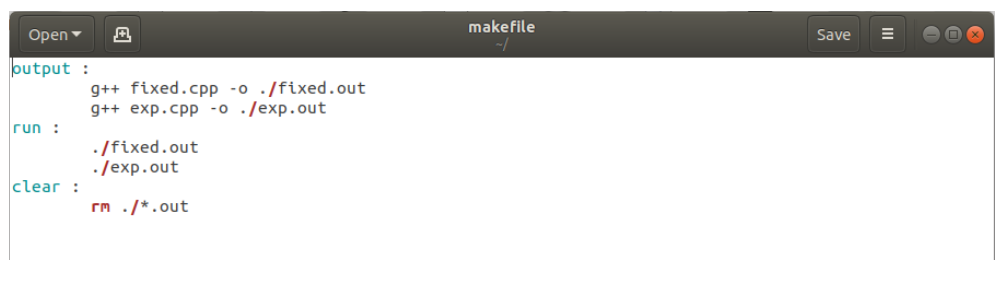
\includegraphics[width=1\textwidth]{Content/guide.png}
	\end{center}
	\end{itemize}
\end{document}